\documentclass[UTF8]{article}
% 中文支持
\usepackage[UTF8]{ctex}	
% pdf调用 封面
\usepackage{pdfpages}
% color宏包
\usepackage{color}  
% 导入图片
\usepackage{caption}
\usepackage{graphicx, subfig}
% 防止图片乱跑
\usepackage{float}
% 支持数学符号
\usepackage{amsmath}
% 支持代码块
\usepackage{listings}
% pdf加入大纲
\usepackage{hyperref}
% 大纲去红框
\hypersetup{hidelinks,
	colorlinks=true,
	allcolors=black,
	pdfstartview=Fit,
	breaklinks=true
}

% 绘制三线表
\usepackage{booktabs}    
% 消除警告
\usepackage{lmodern}

% 绘图
\usepackage{tikz}
\usetikzlibrary{positioning, shapes.geometric}
\tikzstyle{bag} = [align=center]

% 设置页面的环境,a4纸张大小,左右上下边距信息
\usepackage[a4paper, left=31.8mm, right=31.8mm, top=25.4mm, bottom=25.4mm]{geometry}

% 代码块的基本设置
\lstset{
 breaklines,%自动换行
 columns=fixed,       
 numbers=left,                                        % 在左侧显示行号
 numberstyle=\tiny\color{gray},                       % 设定行号格式
 frame=none,                                          % 不显示背景边框
 backgroundcolor=\color[RGB]{245,245,244},            % 设定背景颜色
 keywordstyle=\color[RGB]{40,40,255},                 % 设定关键字颜色
 numberstyle=\footnotesize\color{darkgray},           
 commentstyle=\it\color[RGB]{0,96,96},                % 设置代码注释的格式
 stringstyle=\rmfamily\slshape\color[RGB]{128,0,0},   % 设置字符串格式
 showstringspaces=false,                              % 不显示字符串中的空格
 language=python,                                        % 设置语言
}

% \begin{titlepage}
% % 封面信息
% 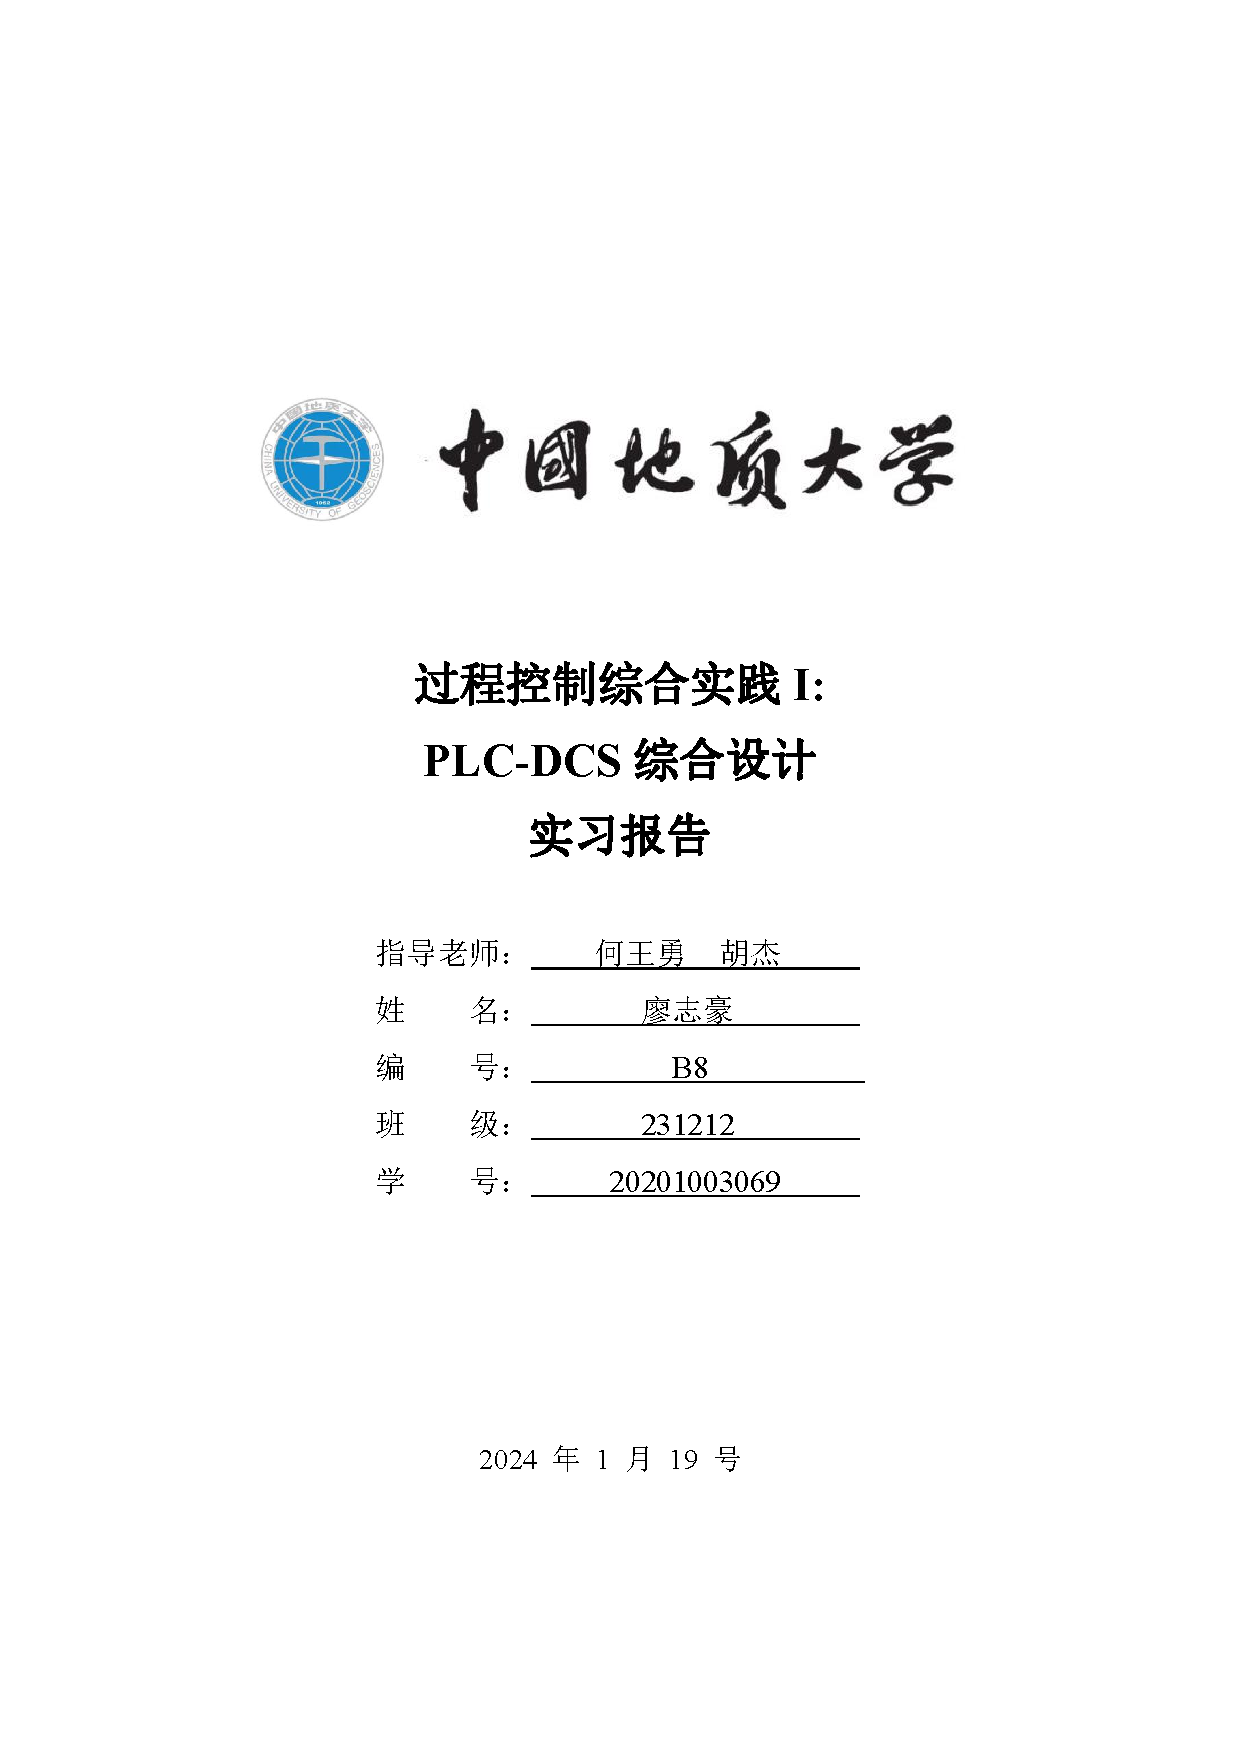
\includepdf[pages={1}]{cover.pdf}
% \end{titlepage}

% 生成目录
% \tableofcontents
% \cleardoublepage

% 导入图片
% \begin{figure}[H]
%     \centering % 居中 
%     % 图片文件的相对路径
%     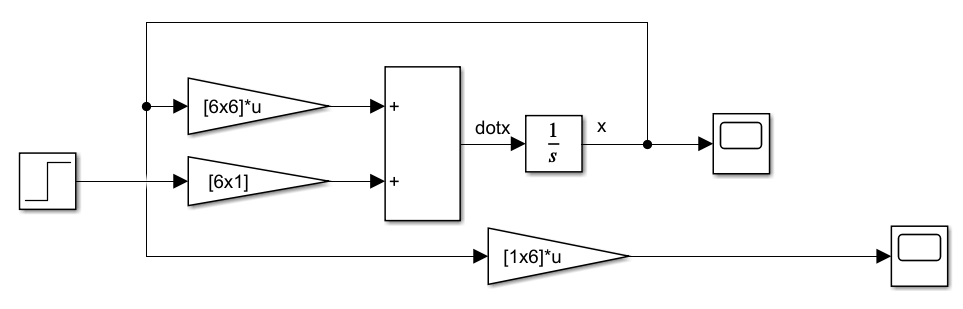
\includegraphics[width=.8\textwidth]{figure/exp1_1_model.png} 
%     \caption{Simulink模型} % caption是图片的标题
%     % \label{img} % 此处的label相当于一个图片的专属标志,目的是方便上下文的引用
% \end{figure}

% 导入代码
% \begin{lstlisting}
% a
% \end{lstlisting}

\begin{document}

% 实验报告主要包含内容:
% (1)实验目的
% (2)实验环境介绍:主要说明针对对象的那一部分进行控制,需要给出简单的模型图结合说明;并指出采取的控制工具和手段(PLC的配置+传感器+执行器)
% (3)实验内容:含工艺流程图和控制框图、原理性分析(主要指控制器正反作用选取、控制策略选取依据);无需对编程内容做详细介绍,实习报告中已体现。
% (4)==重要== 实验结论:PID参数+曲线。重在展示结论与课程原理的对应。

\begin{titlepage}
% 封面信息
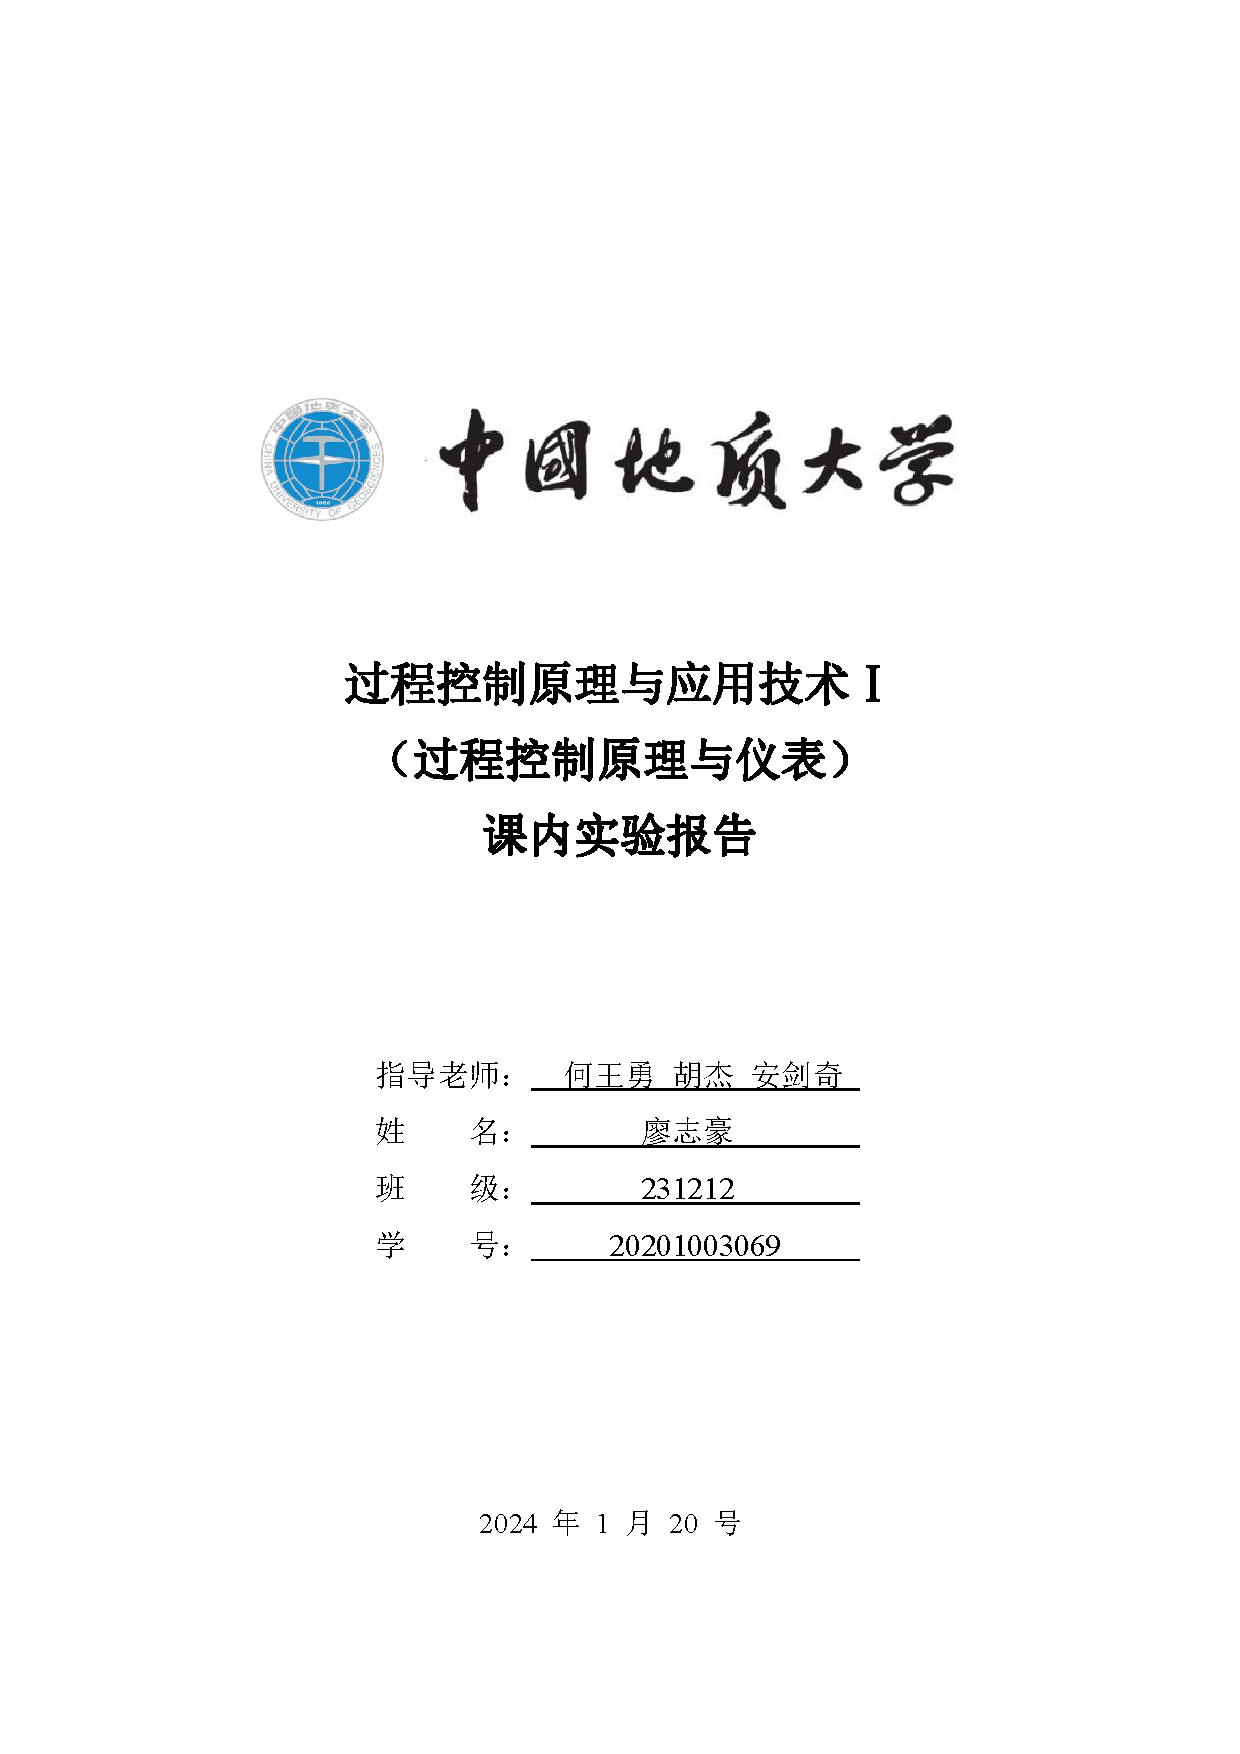
\includepdf[pages={1}]{./cover/cover.pdf}
\end{titlepage}

% 生成目录
\tableofcontents
\cleardoublepage


%
\section{实验一:对象特性分析与过程控制系统结构设计}
%%
\subsection{实验目的}
\begin{enumerate}
	\item 掌握工业过程系统典型被控对象的动态特性分析和测试方法;
	\item 掌握检测仪表、执行机构、PLC控制器的使用方法;
	\item 掌握基于PLC的过程控制系统的软硬件设计。
\end{enumerate}

%%
\subsection{实验环境介绍}
本实验所用的主要设备有:
西门子S7-1200可编程逻辑控制器件,搭配各种辅助设备如交换机、台达显示屏(触摸屏),电源等。

西门子水箱实验台,包含了主、副两个水箱、一个变频器和变频电机、一个工频电机、一个电磁阀、两个液位变送器、两个流量变送器、两个压力变送器,以及若干手动阀。

此外,还需要一台安装有博图软件(建议v15.1以上)的带有网口或配备USB扩展网口的计算机。

%%
\subsection{实验内容}
本次实验的内容如下:
\begin{enumerate}
	\item 设计以水箱为典型对象构建过程控制硬件系统;
	\item 完成包括检测仪表、执行机构、PLC控制器的控制系统通道;
	\item 测试和理解对象的动态特性。
\end{enumerate}

%%
\subsection{过程控制硬件系统搭建}
%%%
\subsubsection{水箱实验台}
本次实验中以水箱实验台作为实验对象,包含了主副两个水箱,每个水箱均有单独的出水阀门和进水管道;实验台提供了工频泵和变频泵用来向水箱供水,且每个泵都可以通过设置相应的手动阀来决定向主副水箱的其中一个供水;除此之外,实验台还提供了多种传感器用于检测水箱系统运行过程中的各种数据,这些传感器包括用来检测主副水箱液位的液位变送器,检测工频段和变频段水流管道流量的流量变送器,以及负责检测压力的压力变送器等。

水箱实验台实物结构图如下所示:
\begin{figure}[H]
    \centering % 居中 
    % 图片文件的相对路径
    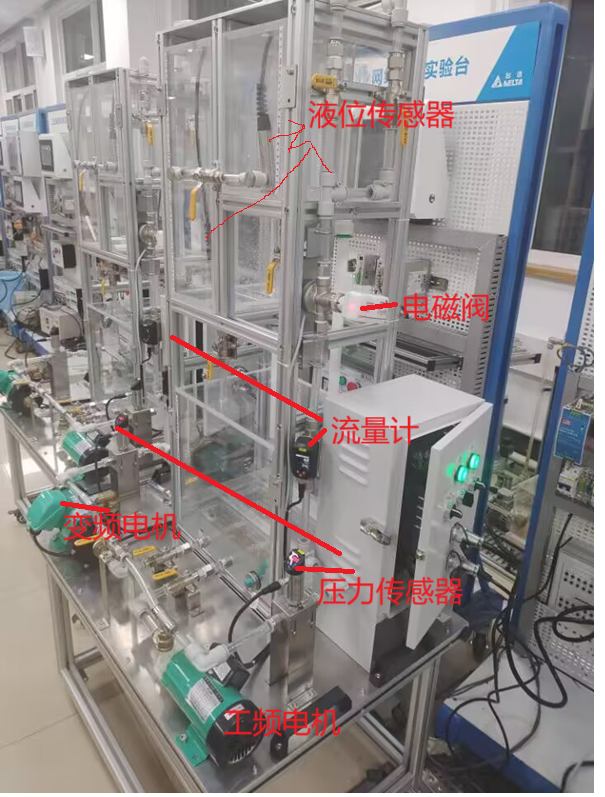
\includegraphics[width=.6\textwidth]{figure/水箱实验台实物结构图.png} 
    \caption{水箱实验台实物结构图} % caption是图片的标题
    % \label{img} % 此处的label相当于一个图片的专属标志,目的是方便上下文的引用
\end{figure}

结合水箱实验台实物结构图可以非常直观的理解水箱系统的工作原理,即水泵通过下面的储水箱将水抽至上面的主副水箱中,并通过水箱下方的管道重新流入储水箱,通过设置手动阀门的开度可以调节水流流入储水箱的流量大小。

%%%
\subsubsection{PLC现场控制单元}
本次实验使用西门子S7-1200 PLC作为水箱系统的现场控制单元,搭配了对应的西门子输入/输出IO模块。PLC现场控制单元的实物图如下所示:
\begin{figure}[H]
    \centering % 居中 
    % 图片文件的相对路径
    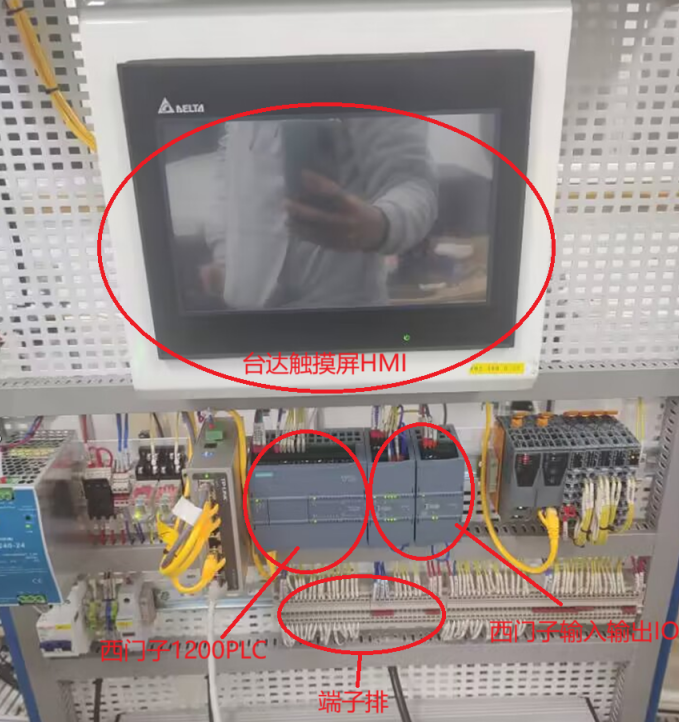
\includegraphics[width=.6\textwidth]{figure/PLC现场控制单元实物图.png} 
    \caption{PLC现场控制单元实物图} % caption是图片的标题
    % \label{img} % 此处的label相当于一个图片的专属标志,目的是方便上下文的引用
\end{figure}

在博图软件中配置其设备组态如下图所示:
\begin{figure}[H]
    \centering % 居中 
    % 图片文件的相对路径
    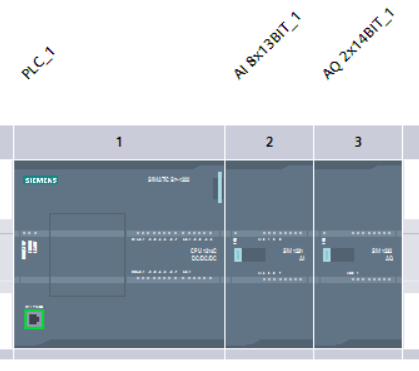
\includegraphics[width=.6\textwidth]{figure/PLC设备组态.png} 
    \caption{PLC设备组态} % caption是图片的标题
    % \label{img} % 此处的label相当于一个图片的专属标志,目的是方便上下文的引用
\end{figure}

%%%
\subsubsection{控制系统分析}
%%%%
\paragraph{执行器的正反作用分析}~{}

水箱实验台一共提供了两个执行器,即变频泵和电磁阀,此外还提供了一个工频泵,由于工频泵我们无法设置其工作频率,故这里不将它作为执行器考虑。对于变频泵,其输入给定值为变频电机的工作频率(实际上存在一个比例关系,成正比),故变频泵是一个正作用执行器,从控制系统的角度考虑,它的放大系数为正;而对于电磁阀,经过使用后我们发现,阀门的开度与其输入给定值的大小是相反的,即输入信号越小,阀门开度越大,故电磁阀这一执行器的作用方式为反作用,其放大系数为负。

%%%%
\paragraph{被控过程正反作用分析}~{}

在本实验中,将水箱作为典型对象进行控制系统设计,故水箱是被控对象,其液位作为被控量。以典型的单容水箱为例,当供水管道水流流量越大,则通常情况下水箱的液位会越高,故可以认为这一被控过程为正作用;对于双容水箱,其分析过程与上述单容水箱类似,在通常情况下也为正作用。

%%%%
\paragraph{控制器正反作用选取}~{}

对于闭环控制系统,其控制器的正反作用选取需要遵循一个原则,即系统中各环节放大系数的乘积为正,只有这样才能构成一个负反馈控制系统。经过上面的分析可以知道水箱实验台中各种执行器以及被控过程的正反作用类型,其中被控过程一般可以认为是正作用。此外实验台所用的各种传感器如液位变送器、流量变送器等均与通常情况下保持一致,其放大系数为正。因此,控制系统中控制器正反作用的选取主要参考执行器的正反作用类型即可。例如,在针对水箱液位的单回路控制系统中,若选取变频泵为执行器,则控制器需要为反作用控制器,其放大系数为正,可以保证闭环系统中各环节的放大系数乘积为正值;若选择电磁阀作为执行器,则控制器设为正作用即可,其放大系数为负值。

%%
\subsection{水箱对象动态特性分析及系统辨识}
%%%
\subsubsection{水箱对象动态特性分析}
如图所示为单容水箱的简单模型示意图。通过阀门1向水箱供水,水箱中的水通过阀门2流出,其中$q_1$为供水流量,可以通过阀门1调节;$q_2$为出水流量,可以通过阀门2调节。水箱的容量系数(横截面积)设为C。
\begin{figure}[H]
    \centering % 居中 
    % 图片文件的相对路径
    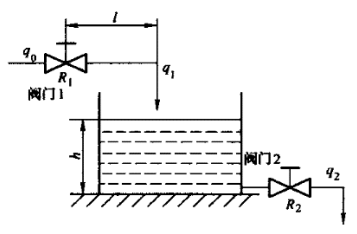
\includegraphics[width=.6\textwidth]{figure/单容水箱模型.png} 
    \caption{单容水箱模型} % caption是图片的标题
    % \label{img} % 此处的label相当于一个图片的专属标志,目的是方便上下文的引用
\end{figure}

由动态物料平衡关系,即液体存储量的变化率 = 单位时间内液体流入量 - 单位时间内液体流出量,得到:
\begin{equation*}
	\Delta q_1 - \Delta q_2 = C\frac{d\Delta h}{dt}
\end{equation*}

假设液体流出量q与液位h近似呈线性正比关系,与阀门液阻R呈反比关系,即液体流出的流量只与出水口处阀门的静压有关,则可以得到:
\begin{equation*}
	\Delta q_2 = \frac{\Delta h}{R_2}
\end{equation*}

将上述各式进行整理,可以得到单容水箱的微分方程模型为:
\begin{equation*}
	R_2C\frac{d \Delta h}{dt} + \Delta h = R_2 \Delta q_1
\end{equation*}

经拉氏变换可以得到:
\begin{equation*}
	(R_2Cs + 1)H(s) = R_2Q(s)
\end{equation*}

由此可以看出,单容水箱为一阶对象(惯性环节),其传递函数为:
\begin{equation*}
	G(s) = \frac{H(s)}{Q(s)} = \frac{R_2}{R_2Cs + 1} = \frac{K}{Ts + 1}
\end{equation*}

%%%
\subsubsection{基于单容水箱液位的系统模型辨识}
根据以上分析可以知道,单容水箱为一阶对象。因此可以采用阶跃响应曲线法对该一阶系统的参数进行辨识。

%%%%
\paragraph{辨识数据采集}~{}

基于变频泵为主水箱供水,主水箱出水口的阀门保持一定开度,使用简单的PID闭环控制将主水箱液位控制在20cm高度处并保持稳定,读取此时的变频泵输入给定值并记录。将闭环控制改为手动开环控制方式,然后将变频泵的输入改为上述记录的给定值,使得主水箱液位在开环控制方式下稳定在20cm高度处。

待主水箱液位稳定后,对变频泵输入一个阶跃信号,即将变频泵输入给定值增大,由于水箱是一个自衡系统,这时主水箱液位将会逐渐自衡到新的高度。在这一过程中,使用PLC以固定的采样时间0.3s记录主水箱的液位数据,并导出至MATLAB中进行分析。

%%%%
\paragraph{基于MATLAB系统辨识工具箱进行水箱系统辨识}~{}

通过理论分析可以知道,单容水箱通常是一个无滞后的一阶对象,其传递函数一般可以表示为:
\begin{equation*}
	G(s) = \frac{K}{Ts + 1}
\end{equation*}

然而,在我们使用的实际水箱系统中,往往会由于水流管道等各种原因导致系统出现一定程度的纯滞后现象。因此,这里将实际单容水箱系统当做一个具有纯滞后的一阶对象,其传递函数可以表示为:
\begin{equation*}
	G(s) = \frac{K\cdot e^{-\tau s}}{Ts + 1}
\end{equation*}

使用MATLAB软件中自带的系统辨识工具箱,对基于上述具有纯滞后的一阶对象传递函数模型进行主水箱系统参数辨识,使用的数据包括水箱液位变化数据以及对应的阶跃信号输入,如下图所示:
\begin{figure}[H]
    \centering % 居中 
    % 图片文件的相对路径
    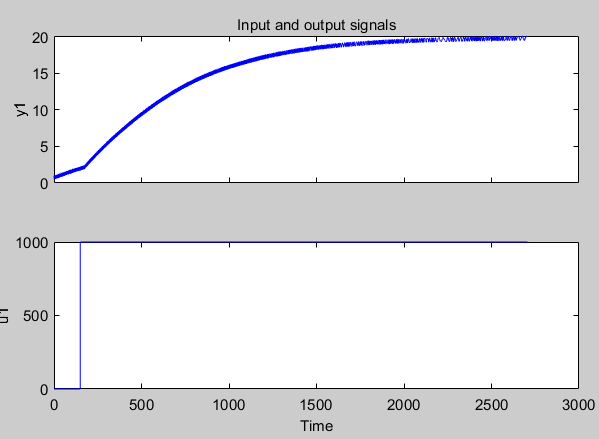
\includegraphics[width=.6\textwidth]{figure/水箱辨识-辨识所用数据.png} 
    \caption{水箱系统辨识所用数据} % caption是图片的标题
    % \label{img} % 此处的label相当于一个图片的专属标志,目的是方便上下文的引用
\end{figure}

%%%%
\paragraph{水箱系统辨识结果}~{}

MATLAB系统辨识工具箱的辨识结果截图如下:
\begin{figure}[H]
    \centering % 居中 
    % 图片文件的相对路径
    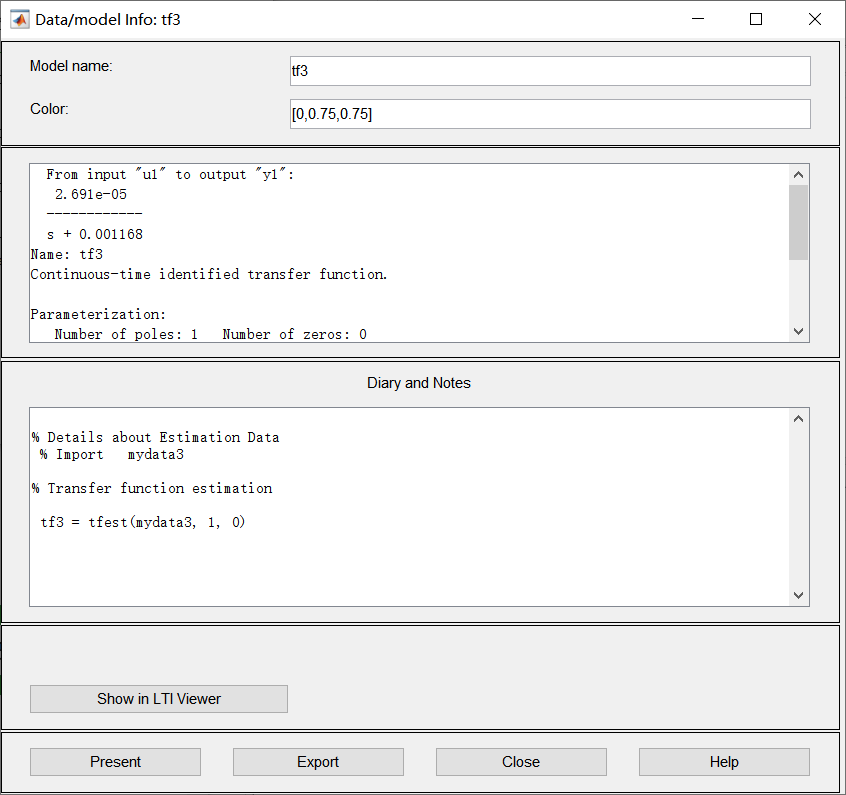
\includegraphics[width=.6\textwidth]{figure/水箱辨识-传递函数.png} 
    \caption{辨识结果截图} % caption是图片的标题
    % \label{img} % 此处的label相当于一个图片的专属标志,目的是方便上下文的引用
\end{figure}

辨识结果的曲线拟合情况如下图所示:
\begin{figure}[H]
    \centering % 居中 
    % 图片文件的相对路径
    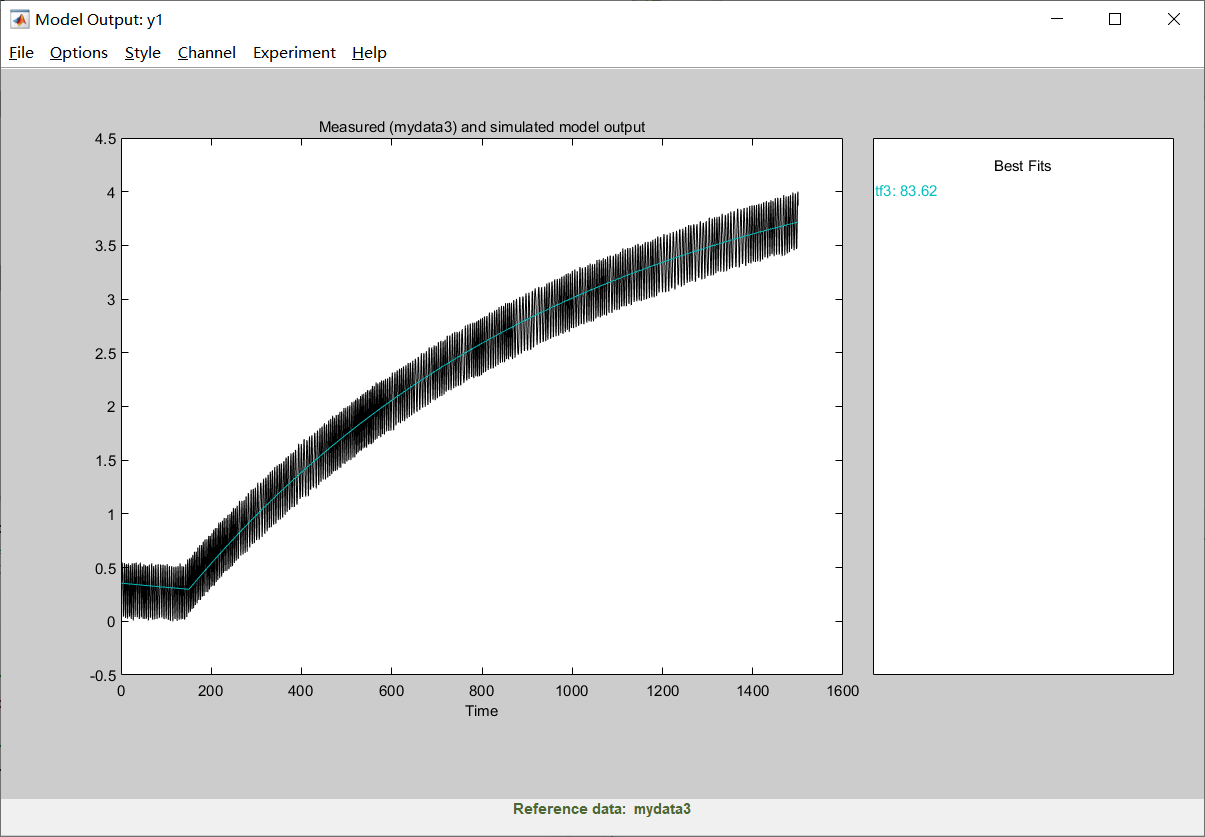
\includegraphics[width=.8\textwidth]{figure/水箱辨识-拟合曲线.png} 
    \caption{辨识结果的曲线拟合情况} % caption是图片的标题
    % \label{img} % 此处的label相当于一个图片的专属标志,目的是方便上下文的引用
\end{figure}

最后得到的单容水箱系统的传递函数模型如下:
\begin{equation*}
	G(s) = \frac{0.02304 \cdot e^{-4.5s}}{856.2s + 1}
\end{equation*}

%%%%
\paragraph{虚拟PID调试}~{}

使用MATLAB软件中的PID调试工具,针对上述单容水箱模型进行PID控制器的调试,最终的控制效果如下图所示:
\begin{figure}[H]
    \centering % 居中 
    % 图片文件的相对路径
    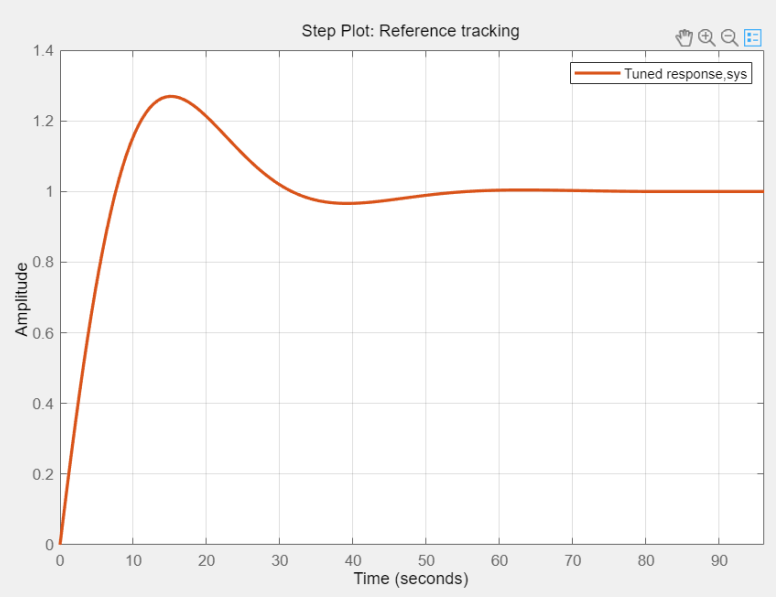
\includegraphics[width=.6\textwidth]{figure/水箱辨识-虚拟pid调试.png} 
    \caption{虚拟PID调试效果图} % caption是图片的标题
    % \label{img} % 此处的label相当于一个图片的专属标志,目的是方便上下文的引用
\end{figure}

%%
\subsection{实验结论}

在本次实验中,我们首先对实验所用的过程控制硬件设备进行了分析。对于水箱实验台,我们分析了其包含的各种可能的被控对象,如单容水箱、双容水箱等;然后分析了我们需要用到的各种传感器和执行器设备,以及水箱实验台整体的工作方式和原理。对于本次实验所用的西门子PLC现场控制单元,我们探究了其所拥有的IO口模块等资源,并对PLC设备组态、网络通讯等进行了配置。在这个过程中,我们熟悉了整个水箱控制系统的工作原理和运行方式。

针对水箱对象的动态特性分析以及系统辨识,我们首先通过理论分析和推导的方式得出了结论,即单容水箱为一个典型的一阶对象,并且在实际场景中,还需要考虑其纯滞后的特性。基于以上理论分析得到的单容水箱模型,我们利用实测数据对主水箱液位进行了水箱模型的系统辨识,并得到了主水箱的传递函数。



\newpage
%
\section{实验二:PID控制器设计与参数整定}
%%
\subsection{实验目的}
\begin{enumerate}
	\item 掌握单回路系统分析和设计方法;
	\item 掌握PID控制器各参数的控制作用与整定方式;
	\item 理解对象和控制器的变化对控制效果的影响。
\end{enumerate}

%%
\subsection{实验对象介绍}

针对水箱实验台的主水箱部分进行控制,主水箱作为控制对象,变频泵作为执行器,主水箱液位变送器为检测设备。其中主水箱液位为被控量,变频器工作频率为控制量,并使用基于西门子S7-1200 PLC的PID控制器构成一个单回路闭环控制系统。

% 针对水箱实验台的主水箱部分进行控制,以主水箱作为被控对象,主水箱液位为被控量,

% 对于单回路控制系统设计,我们选择主水箱作为控制对象,变频泵作为执行器,主水箱液位变送器为检测设备。其中主水箱液位为被控量,变频器工作频率为控制量,并使用PID控制器构成单回路闭环控制系统。主水箱液位控制系统框图如下所示:

%%
\subsection{实验内容}
\begin{enumerate}
	\item 以水箱为对象,设计PID单回路控制系统;
	\item 整定PID参数,理解各参数的作用;
	\item 分析和对比不同水箱,不同PID参数的控制效果。
\end{enumerate}

%%
\subsection{PID单回路控制系统设计}

%%%
\subsubsection{PID控制器原理介绍}
常用的位置式PID控制器的计算公式如下:
\begin{align*}
	u(t) &= K_ce(t) + \frac{K_c}{T_I}\int_0^t e(t)dt + K_cT_D\frac{de(t)}{dt} \\
	&= K_p \cdot e(t) + K_i \cdot \int_0^t e(t)dt + K_d \cdot \frac{de(t)}{dt}
\end{align*}

其数字形式可以表示为:
\begin{equation*}
	u(k) = K_p \cdot e(k) + K_i \cdot \sum e(k) + K_d \cdot [e(k) - e(k-1)]
\end{equation*}

PID控制器中各个参数的作用各有不同:
\begin{itemize}
	\item $K_p$:比例作用用于加快系统的响应速度,减小系统的稳态误差。$K_p$越大,系统的响应速度越快,调节精度越高,但会导致超调量增大,使得系统稳定性降低;$K_p$过小,会降低调节精度,使响应速度变慢,从而延长调节时间,系统动态性能变差。
	\item $K_i$:积分作用主要用来消除静差,提高系统的无差度。增大$K_i$可以提高系统的响应速度,但是由于系统的相角发生滞后,会导致系统的动态特性变差,容易引发系统振荡。当$K_i$过大时,会容易导致系统在响应过程中出现积分饱和现象,使控制系统暂时失去调节能力,因此通常需要搭配积分限幅、积分分离等手段。
	\item $K_d$:微分作用能改善系统的动态特性,提高系统的稳定性。微分作用主要根据偏差的变化趋势提前进行调节,以避免系统出现过大的超调量。此外,微分作用对高频信号比较敏感,不适合用于变化比较剧烈的过程中,如对流量、压力等参数的控制,而且当系统中包含高频噪声时也不适合引入微分作用。
\end{itemize}

%%%
\subsubsection{主水箱液位单回路控制系统设计}
对于单回路控制系统设计,我们选择主水箱作为控制对象,变频泵作为执行器,主水箱液位变送器作为检测设备。其中主水箱液位为被控量,变频器工作频率为控制量,水箱出水口流量为干扰量,并使用PID控制器构成单回路闭环控制系统。主水箱液位控制系统框图如下所示:
\begin{figure}[H]
    \centering % 居中 
    % 图片文件的相对路径
    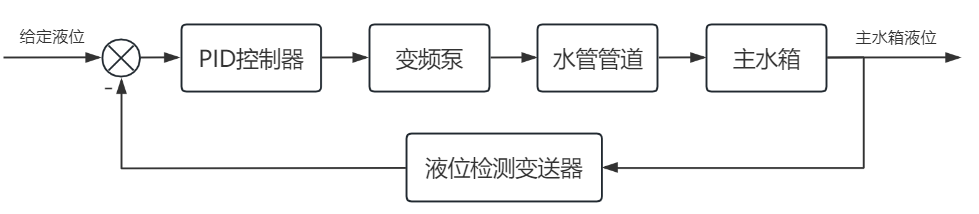
\includegraphics[width=.8\textwidth]{figure/主水箱液位单回路控制系统框图.png} 
    \caption{主水箱液位单回路控制系统框图} % caption是图片的标题
    % \label{img} % 此处的label相当于一个图片的专属标志,目的是方便上下文的引用
\end{figure}

%%%%
\paragraph{控制策略选取}~{}

在水箱液位单回路控制系统设计中,我们选择了比例-积分(PI)控制策略。在实验过程中,我们发现液位变送器检测到的液位数据存在高频的波动(参考我们在水箱系统辨识时所用的液位数据),因此在这一控制系统设计中不宜引入微分作用。


%%
\subsection{PID参数整定}
%%%
\subsubsection{PID参数整定方法}
在实验过程中,我们最常使用的PID参数整定方法是根据经验来调整参数,比如下面的PID参数整定口诀:
\begin{figure}[H]
    \centering % 居中 
    % 图片文件的相对路径
    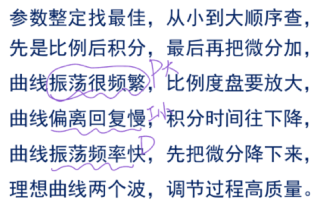
\includegraphics[width=.4\textwidth]{figure/PID参数整定口诀.png} 
    \caption{PID参数整定口诀} % caption是图片的标题
    % \label{img} % 此处的label相当于一个图片的专属标志,目的是方便上下文的引用
\end{figure}

应当注意,在对PID控制器进行参数调试时,应该遵守“先比例,后积分,再微分”的引入顺序。此外我们还使用了从课上学习到的针对单回路控制系统的PID控制器参数整定方法,如临界比例度法和衰减曲线法,下面分别对它们进行介绍。

%%%%
\paragraph{临界比例度法}~{}

临界比例度法又称稳定边界法,是一种闭环参数整定方法,其整定步骤大致如下:
\begin{enumerate}
    \item 将控制器的积分时间$T_I$置于最大,微分时间$T_D$置零,比例带$\delta$置为较大的数值,使系统投入闭环运行。
    \item 系统运行稳定后,对设定值施加一个阶跃扰动,并减小比例度$\delta$直到系统出现等幅振荡为止,即临界振荡过程。记录此时的临界比例带$\delta$与等幅振荡周期$T_K$。利用记录的数据,根据经验公式就可计算出控制器参数。
\end{enumerate}

经验公式如下表所示:
\begin{table}[H] % 防止表格乱跑
\centering % 居中
\begin{tabular}{cccccc} % 指明列数
	\toprule % 顶部粗线
    控制规律 & $\delta$ & $T_I$ & $T_D$ \\
	\midrule % 中间细线
	P & $2\delta_K$ & - & - \\
    PI & $2.2\delta_K$ & $0.85T_K$ & - \\
    PID & $1.66\delta_K$ & $0.5T_K$ & $0.125T_K$ \\ 
	\bottomrule % 底部粗线
\end{tabular}
\caption{临界比例度法经验公式} % 标题
\end{table}

%%%%
\paragraph{衰减曲线法}~{}

衰减曲线法与临界比例度法类似,不同的是衰减曲线法不需要系统出现等幅振荡。其具体步骤大致如下:
\begin{enumerate}
    \item 将控制器的积分时间$T_I$置于最大,微分时间$T_D$置零,比例带$\delta$置为较大的数值,使系统投入闭环运行。
    \item 系统运行稳定后,对设定值施加一个阶跃扰动,然后观察系统的响应。若响应曲线振荡频繁,就增大比例带;反之则减小比例带。如此反复,直至系统出现衰减比为$n = 4:1$或$n = 10:1$的响应曲线,记录此时的比例带$\delta_K$,以及相应的衰减震荡周期$T_s$($n = 4:1$)或者上升时间$T_r$($n = 10:1$)。
    \item 根据记录的数据,按照经验公式计算出控制器的参数。
\end{enumerate}

衰减曲线法的经验公式如下所示:
\begin{figure}[H]
    \centering % 居中 
    % 图片文件的相对路径
    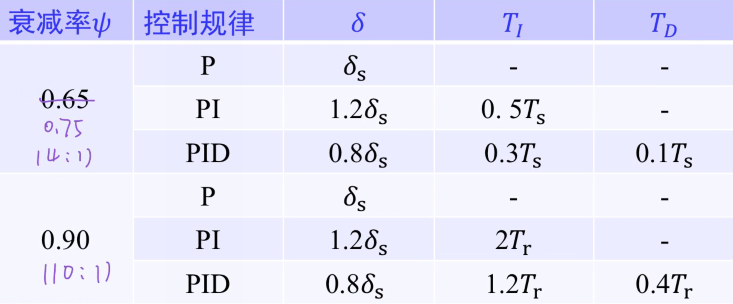
\includegraphics[width=.6\textwidth]{figure/衰减曲线法经验公式.png} 
    \caption{衰减曲线法经验公式} % caption是图片的标题
    % \label{img} % 此处的label相当于一个图片的专属标志,目的是方便上下文的引用
\end{figure}

%%%
\subsubsection{参数整定结果}
经参数整定后,最终使用的PID控制器各参数如下:
\begin{figure}[H]
    \centering % 居中 
    % 图片文件的相对路径
    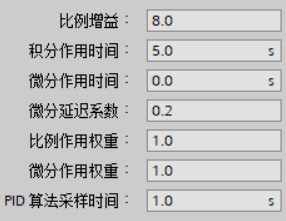
\includegraphics[width=.4\textwidth]{figure/单回路-模块-PID参数.png} 
    \caption{单回路控制器参数} % caption是图片的标题
    % \label{img} % 此处的label相当于一个图片的专属标志,目的是方便上下文的引用
\end{figure}

%%%
\subsubsection{控制效果展示}
主水箱液位单回路控制系统的控制效果如下所示:
\begin{figure}[H]
    \centering % 居中 
    % 图片文件的相对路径
    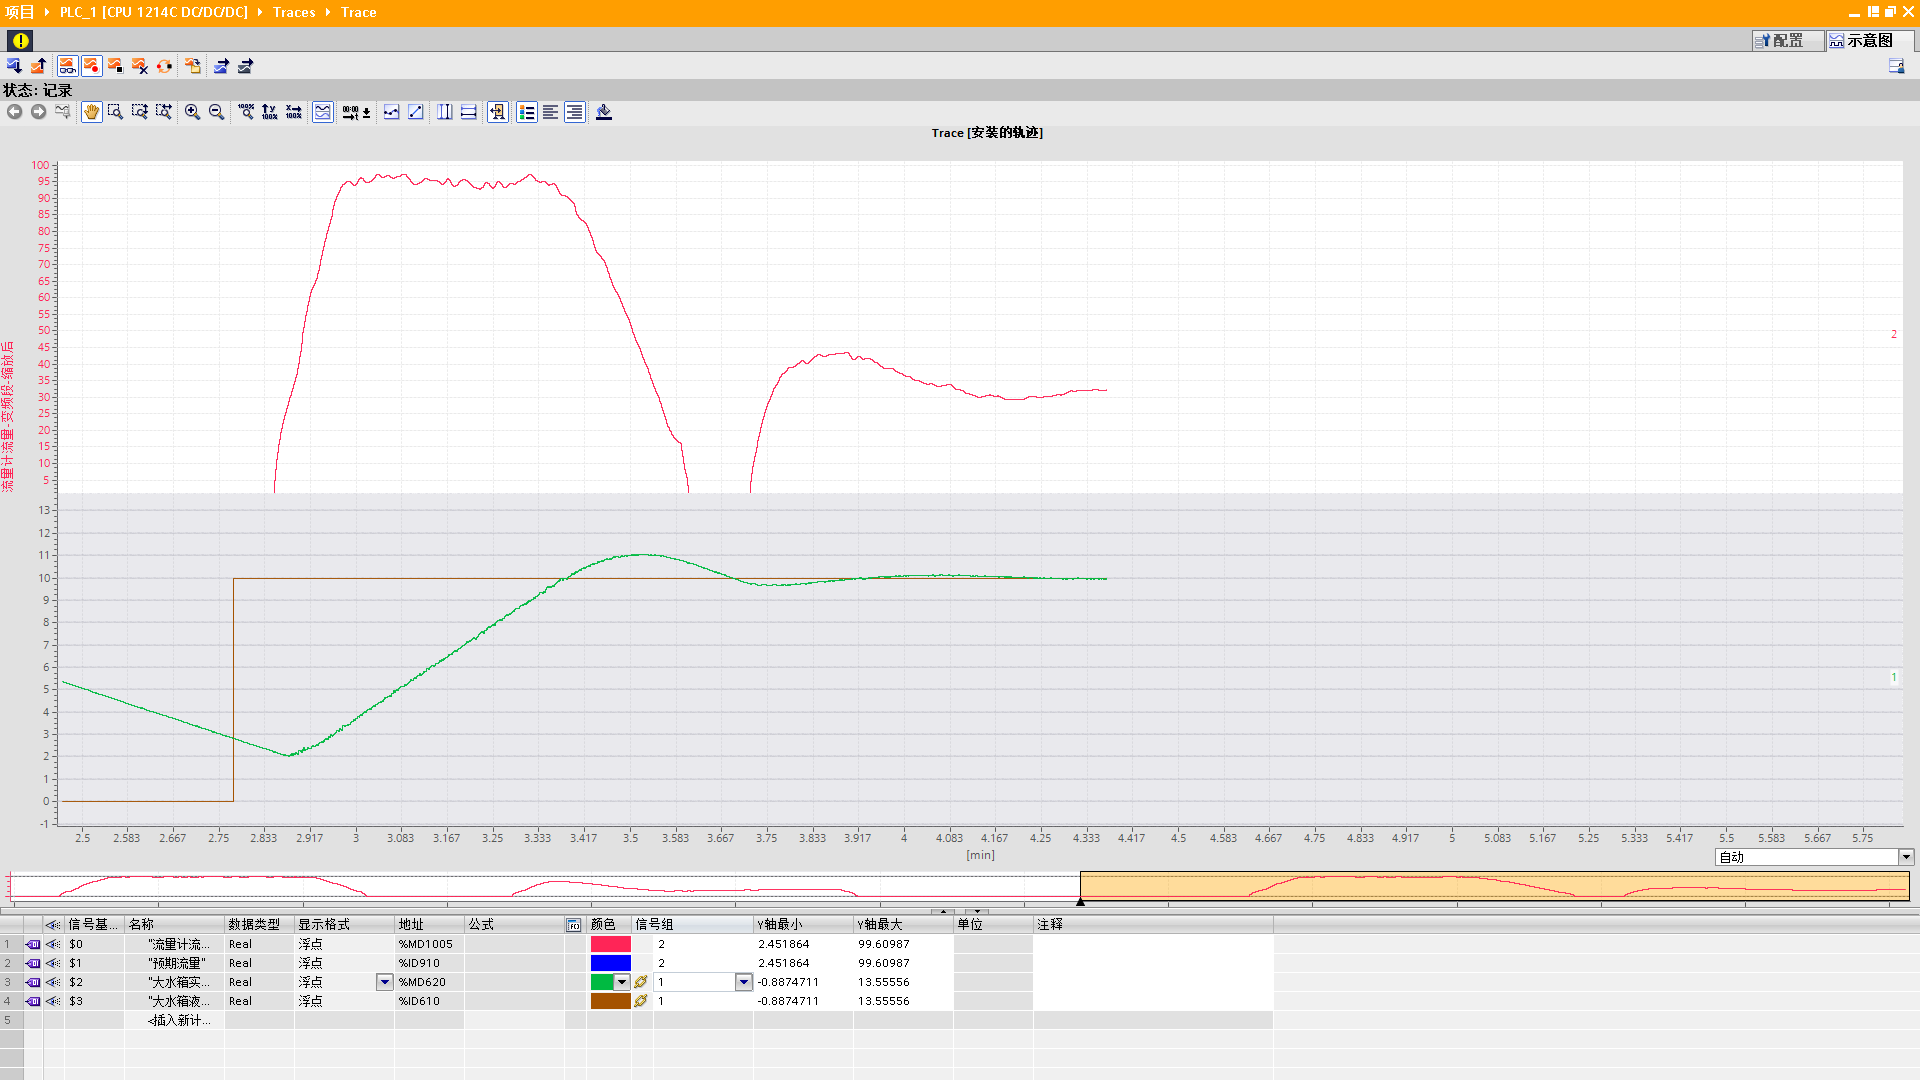
\includegraphics[width=1\textwidth]{figure/单回路控制效果-模块.png} 
    \caption{主水箱液位单回路控制效果} % caption是图片的标题
    % \label{img} % 此处的label相当于一个图片的专属标志,目的是方便上下文的引用
\end{figure}
其中,绿色曲线代表主水箱实际液位,棕色曲线代表主水箱液位给定值,红色曲线代表变频段管道流量值。可以看到,主水箱实际液位的调节曲线出现了幅值比例约4:1的两个波峰,符合控制要求。

%%
\subsection{实验结论}
% - PID参数 + 曲线
% - 结论与课程原理的对应

在这次实验中,我们针对主水箱液位设计了一个单回路闭环控制系统。通过这个过程我们进一步体会到了PID算法的运行原理,即根据给定值与实际测量值之间的偏差,通过比例、积分、微分等运算后,将得到的控制量施加到执行器上,以此完成对被控变量的调节过程。在对PID控制器进行参数整定的过程中,我们也加深了对PID控制器各参数作用的理解,同时学会了如何利用理论知识对PID控制器的参数进行调整,掌握了单回路PID控制器的设计和一些工业上常用的参数整定方法,可以说获益良多。

% 系统控制器的设计部分结束,在此过程中,我对被控对象的特性做出了分析,辨识出系统参数,熟悉了整个水箱的液位控制过程。通过水箱中液位变送器的实时反馈数据来得到偏差值,通过偏差来对系统进行控制,使得水箱液位保持稳定。在设计的过程中,我加深了对 PID 控制器在实际场景下应用的理解,掌握了单回路控制系统与串级控制系统在应用时如何抉择,以及在考虑问题时应该首先分析系统的工艺流程,再明确被控对象是什么,可用的控制手段有什么,最后再将各个部分联系在一起,设计适合控制目标的控制系统。在此过程之中,我受益良多。

% 在这一次的实验中,我加深了对单回路 PID 参数整定方法的理解,基本掌握了单回路PID 参数的整定方式。通过对水箱中液位的控制,我学到了如何去应用理论知识来整定 PID控制器的各项参数。在实践的过程中,通过经验法的辅助,我们很快的调出了衰减比为 4:1的响应曲线,调整完成后,我对 PID 控制器的参数整定有了更加直观的理解与感受。我相信在之后的 PID 参数整定的相关内容我都可以很快的解决它们。在此之后,我们还思考了不同PID 参数的效用,对比了不同水箱之间的差异之处,明白了同一组 PID 控制器参数一般不能对不同系统混用,混用很难达到同样强度的控制效果。



\newpage
%
\section{实验三:串级控制系统设计与分析}
%%
\subsection{实验目的}
\begin{enumerate}
	\item 掌握复杂被控对象的分析方法;
	\item 掌握串级控制系统结构的设计方法;
	\item 掌握串级系统内外环的设计方法。
\end{enumerate}

%%
\subsection{实验环境介绍}
% - 被控对象
% - 控制工具和手段 传感器 执行器

在本次串级控制系统设计中,我们选择以水箱实验台的主、副水箱组成的双容水箱作为被控对象,其中主水箱液位作为主被控量,副水箱液位为副被控量。所需的传感器包括主水箱液位变送器、副水箱液位变送器,所需执行器为变频泵。

%%
\subsection{实验内容}
\begin{enumerate}
	\item 以多容水箱为对象,设计串级控制系统结构,理解内外环的作用;
	\item 设计主/副控制器算法,理解主/副控制器作用;
	\item 分析和对比单回路控制系统,理解串级控制系统的优势。
\end{enumerate}

%%
\subsection{双容水箱液位串级控制系统设计}
%%%
\subsubsection{串级控制系统简介}
%%%%
\paragraph{串级控制系统结构和内外环作用分析}~{}

串级控制由两个或以上的控制器串联形成,其中一个控制器的输出作为另一个控制器的设定值。与单回路控制系统相比,串级控制系统增加了一个检测变送单元和一个控制器,从而在结构上形成了两个闭环。里面的闭环称为副回路,它是一个随动系统;外面的闭环称为主回路,它是一个定值控制系统。一个典型串级控制系统的结构框图如下图所示:
\begin{figure}[H]
    \centering % 居中 
    % 图片文件的相对路径
    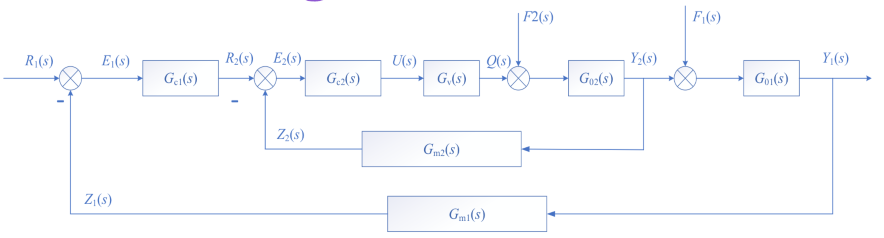
\includegraphics[width=1\textwidth]{figure/串级控制系统典型框图.png} 
    \caption{典型串级控制系统的结构框图} % caption是图片的标题
    % \label{img} % 此处的label相当于一个图片的专属标志,目的是方便上下文的引用
\end{figure}

%%%%
\paragraph{串级控制系统的特点}~{}

串级控制系统由于增加了包含二次干扰的副回路,使得整体的控制效果有了显著的改善。系统对二次干扰有很强的克服能力,进而提高了对一次干扰的克服能力和对外界环境变化的自适应能力;另一方面由于副回路的引入改善了被控过程的动态特性,提高了系统的工作频率。

串级控制系统的主要特点为:
\begin{enumerate}
    \item 对进入副回路的二次干扰有很强的抑制能力;
    \item 能有效改善控制通道的动态特性,提高系统的工作频率;
    \item 对负荷或操作条件的变化有一定的自适应能力。
\end{enumerate}

%%%%
\paragraph{主副控制器作用分析}~{}

主控制器主要负责维持主被控量的稳定性,而副控制器在通常情况下可以认为是为了抑制主要干扰或针对被控过程中的某一干扰进行快速调节而引入的辅助手段。通常可以把副控制器所在的内环当做外环的一个环节来看待,该环节是一个随动系统,通过执行器执行主控制器的调节指令以实现对被控过程中的某一个中间过程参数的控制和调节,进而达到对主被控量进行控制的目的。主副控制器这两者的结合使得控制系统整体能够更好地满足控制需求。

%%%
\subsubsection{双容水箱液位串级控制系统设计}
我们使用了实验台提供的主、副两个水箱构成双容水箱,并将其作为被控对象,设计了一个双容水箱液位串级控制系统。由于主、副水箱之间已经有管道连接,只需将该管道的手动阀打开即可在主、副两水箱之间建立耦合关系。

双容水箱液位串级控制系统的大致思路为:通过控制副水箱的液位以间接控制主水箱的供水流量,从而达到控制主水箱液位的目的。其中,通过设置相应手动阀的开关可以将变频泵的供水引至副水箱中,使得可以通过变频泵调节副水箱液位。在该控制系统中,外环以主水箱液位为主被控量,由主水箱液位变送器进行检测;内环以副水箱液位为副被控量,可通过副水箱液位变送器检测;外环的输出为期望的副水箱液位,实际上与主、副水箱之间水管的流量成正相关关系,外环输出给到内环进行调节,使得副水箱液位可以满足对于流量的需求。双容水箱液位串级控制系统框图如下所示:
\begin{figure}[H]
    \centering % 居中 
    % 图片文件的相对路径
    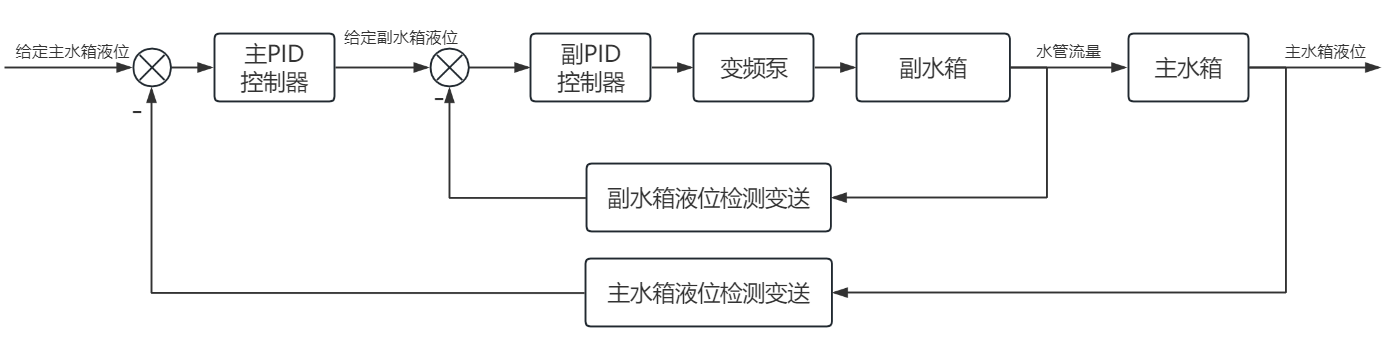
\includegraphics[width=1\textwidth]{figure/双容水箱控制系统框图.png} 
    \caption{双容水箱液位串级控制系统框图} % caption是图片的标题
    % \label{img} % 此处的label相当于一个图片的专属标志,目的是方便上下文的引用
\end{figure}

%%%%
\paragraph{控制策略选取}~{}

在双容水箱液位串级控制系统中,主控制器选为比例-积分(PI)控制,副控制器选择了比例-积分-微分(PID)控制。由于 PI 控制器兼顾了比例控制和积分控制的特点,在可以对误差进行快速响应的同时还能够进一步消除系统可能存在的稳态误差,提高控制精度,是一种使用非常广泛的控制策略。串级控制系统中的内环负责对副水箱液位进行控制,由于实际上副水箱放水的管道管径较小,放水流量受到了很明显的限制,导致了当主控制器输出信号出现较大幅度的下降时,副水箱液位无法很好地对液位给定值进行跟踪。这就意味着对于双容水箱对象的控制,副回路需要满足更高的控制质量要求。综合上述原因,我们结合实验中调试参数得到的经验,最终将副控制器选为PID控制策略。

% 对于主水箱液位-流量串级控制系统,我们选择的主、副控制器的控制策略均为比例-积分(PI)控制策略。这里的内环同样使用了 PI 控制,原因在于我们在实验过程中发现,在仅使用比例控制的情况下流量会出现较大的波动现象,导致水箱液位不能快速稳定下来,而会出现等幅振荡的情况。在对副控制器加入了积分作用以后,情况有了比较明显的改善。

%%%%
\paragraph{主、副控制器正反作用选取}~{}

对于串级控制系统,主、副控制器正反作用方式的选择原则是,使整个控制系统构成负反馈系统,即主通道各环节的放大系数正负极性相乘必须要为正值。

对于本次设计的双容水箱液位串级控制系统,主、副控制器均设置为反作用控制器,原因如下:

在副控制回路中,变频泵作为执行器,经过前面的分析可以知道该环节的放大系数为正;对于副水箱,当变频器的工作频率越高时,则供水水量越大,副水箱的液位也会越高,故副被控过程的放大系数也为正数;此外,对于副水箱液位检测变送器,通常可以将其传递函数看做一个常量(可以简单认为其传递函数为 1),故检测变送环节的放大系数仍为正;综合以上分析,要满足上面的选取原则,则副控制器的放大系数要为正数,即为反作用控制器。

将副回路看做主回路中的一个环节,通过分析不难得出该环节是正作用环节,对于主控制回路,与上述副回路的分析方式类似,可以得到主控制器的放大系数也为正数,即为反作用控制器。


%%%
\subsubsection{串级控制系统参数整定}
在对串级控制系统进行参数整定的过程中,我们参考了课上所学的相关知识,将副回路的工作频率设置为主回路的3$\sim$10倍。此外,我们还借鉴了课堂上介绍的针对串级控制系统的一些PID参数整定方式,如逐步逼近法、两步整定法和一步整定法。这些针对串级控制系统的参数整定方法大多是基于单回路控制系统参数整定方法之上的。

我们在实验过程中主要使用了逐步逼近法和、两步整定法以及经验法来完成初级控制系统的PID控制器参数整定,下面分别对逐步逼近法和两步整定法进行简要介绍。

%%%%
\paragraph{逐步逼近法}~{}

逐步逼近法和经验调参法有一些相似之处,一般适用于主、副过程的时间常数相差不多,主、副回路的动态联系比较紧密的情况。逐步逼近法的大致步骤包括:
\begin{enumerate}
    \item 在主回路开环的情况下,整定副控制器参数;
    \item 使主回路闭合,整定主控制器参数;
    \item 在主回路闭合的情况下,整定副控制器参数,完成一次逼近;
    \item 反复逐步逼近,直到获得满意的控制质量指标为止。
\end{enumerate}

使用逐步逼近法的一个主要缺点在于,参数的整定需要反复进行,以逐步逼近的方式获得最终的调参结果,所以需要花费比较多的时间。但是使用此方法来调节系统有助于我们结合实际系统理解PID控制器各个参数的作用。

%%%%
\paragraph{两步整定法}~{}

两步整定法将副控制器及其所在的副控制回路视为系统的一个环节,在整定好副控制器参数后,对主控制器参数进行整定。其大致步骤如下:
\begin{enumerate}
    \item 整定副控制器的比例度和操作周期:在工况稳定、主副回路闭合情况下,主控制器为纯比例运行,比例度固定在100\%,用4:1衰减曲线法整定副控制器参数,求得副控制器在4:1衰减过程下的比例度$\delta_{2s}$和操作周期$T_{2s}$;
    \item 求取主控制器的比例度和操作时间:在副控制器比例度$\delta_{2s}$的条件下,逐步降低主控制器比例度,求取同样的递减比过程中主控制器的比例度$\delta_{1s}$和操作周期$T_{1s}$;
    \item 计算主、副控制器的比例度,积分时间和微分时间的数值:根据$\delta_{1s},\ \delta_{2s},\ T_{1s},\ T_{2s}$,结合控制器选型,按单回路控制系统衰减曲线法整定参数的经验公式,整定主、副控制器参数;
    \item 必要时进行适当调整,知道系统质量达到最佳为止:按照先副后主、先P次I后D的顺序,将计算出的参数值设置到控制器上,做一些扰动实验,观察过渡过程曲线,适当调整,直至过渡过程质量最佳。
\end{enumerate}

在使用两步整定法整定串级控制系统时,要注意主、副对象的时间参数一般要求为$T_{01}/T_{02} = 3\sim 10$,与前述串级控制系统设计中对控制器的要求一致。此外,在串级控制系统中,一般对主被控量的控制质量要求较高,对副被控量的要求则较低,因此可以允许牺牲一点副被控量的控制质量,比如控制精度的要求可以适当放低。

%%%
\subsubsection{串级控制系统参数整定结果}
经参数整定后,双容水箱串级控制系统的主、副控制回路的PID控制器参数分别如下所示:
\begin{table}[H] % 防止表格乱跑
\centering % 居中
\begin{tabular}{cc} % 指明列数
	\toprule % 顶部粗线
	水箱液主控制回路 & 流量副控制回路 \\
	\midrule % 中间细线
	Kp = 22.0 &  Kp = 6.0\\
	Ki = 0.35 & Ki = 0.1 \\
	Kd = 0.0 & Kd = 0.1 \\
	\bottomrule % 底部粗线
\end{tabular}
\caption{双容水箱串级控制系统PID控制器参数} % 标题
\end{table}

%%%
\subsubsection{控制效果展示}
我们设计的双容水箱液位串级控制系统的控制效果如下图所示:
\begin{figure}[H]
    \centering % 居中 
    % 图片文件的相对路径
    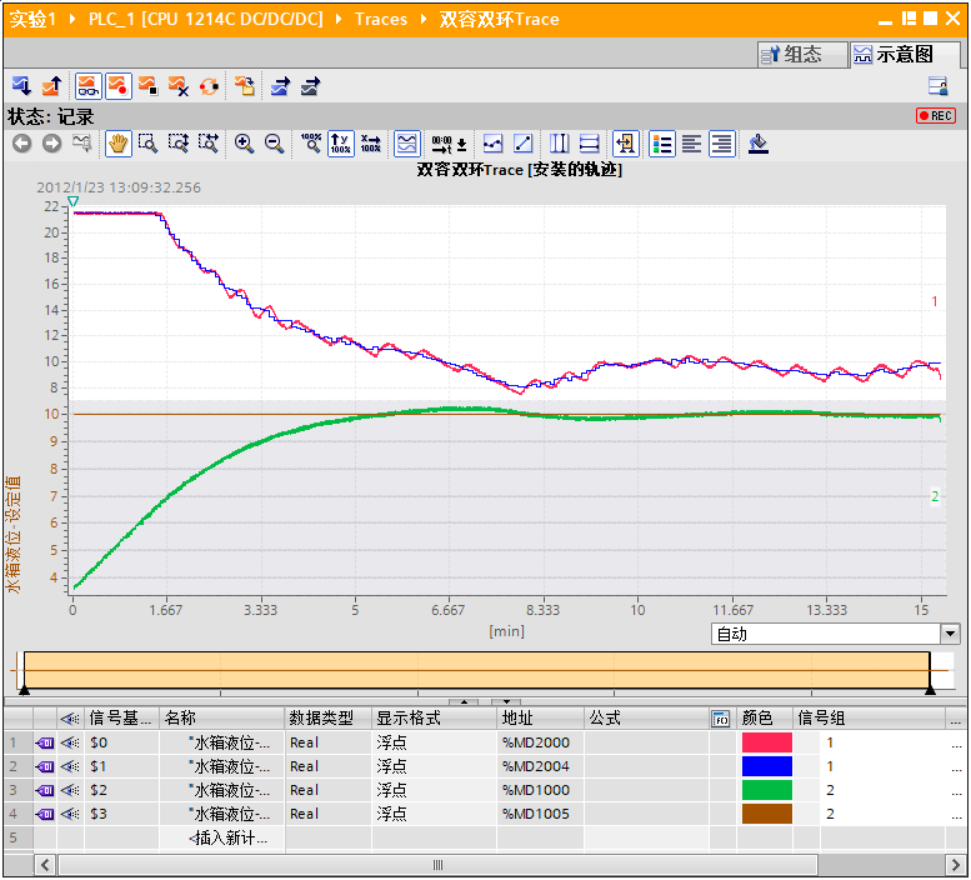
\includegraphics[width=0.8\textwidth]{figure/双容水箱控制效果图.png} 
    \caption{双容水箱液位串级控制系统控制效果} % caption是图片的标题
    % \label{img} % 此处的label相当于一个图片的专属标志,目的是方便上下文的引用
\end{figure}
从上图可以看出,内环所控制的副水箱液位基本可以做到对给定值的跟随。由于主、副水箱之间的水管管径比较小,且副水箱的水箱高度较低,因此该处的水流流量存在比较明显的限制。当给定的副水箱液位值下降过快时,副水箱放水的流量可能无法很好的满足其要求,这是我们在进行双容水箱控制系统设计时发现的一个比较棘手的问题。要解决这一问题,需要在参数整定的过程中注意不要让主控制器的输出(副水箱期望液位)出现大幅度的下降。对此我们的经验之一是不能让系统的响应太快,而要适当放慢响应速度(减小比例系数),否则会容易出现上述问题。

%%
\subsection{主水箱液位-流量串级控制系统设计}
%%%
\subsubsection{液位-流量串级控制系统设计}
除了上述双容水箱液位串级控制系统以外,我们还针对主水箱的液位控制设计了一个液位-流量串级控制系统。这里我们仍选择主水箱作为主要被控对象,主水箱液位为主被控量,将主水箱对应的变频段管道作为副被控对象,其水流流量为副被控量,主副控制器均使用PID控制器。此外,执行器和检测变送器与单回路控制系统均保持一致。系统整体构成一个双闭环的主水箱液位-流量串级控制系统,外环对主水箱液位进行控制,其输出为期望的水管流量,输入到内环;内环根据外环的给定值,对供水的变频段管道流量进行快速调节。主水箱液位-流量串级控制系统框图如下所示:
\begin{figure}[H]
    \centering % 居中 
    % 图片文件的相对路径
    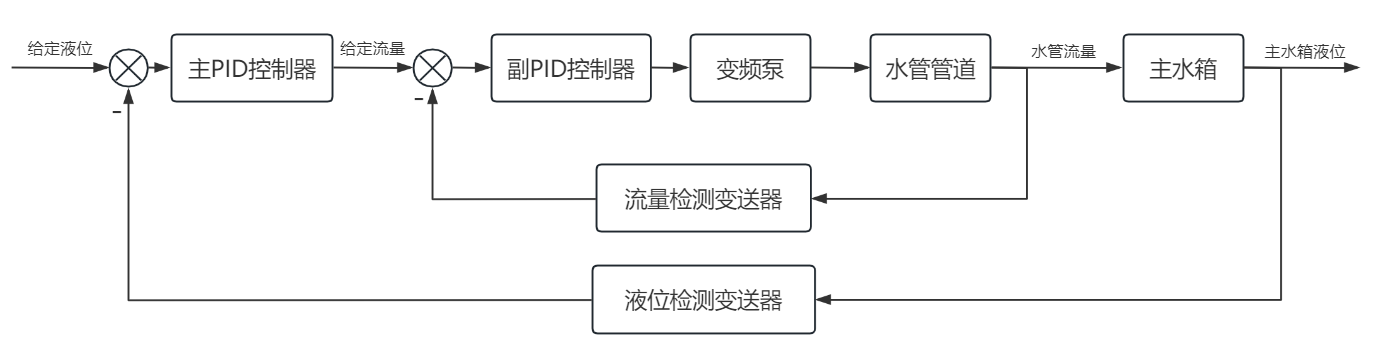
\includegraphics[width=1\textwidth]{figure/主水箱液位-流量串级控制系统框图.png} 
    \caption{主水箱液位-流量串级控制系统框图} % caption是图片的标题
    % \label{img} % 此处的label相当于一个图片的专属标志,目的是方便上下文的引用
\end{figure}

%%%%
\paragraph{控制策略选取}~{}

对于主水箱液位-流量串级控制系统,我们选择的主、副控制器的控制策略均为比例-积分(PI)控制策略。由于PI控制器兼顾了比例控制和积分控制的特点,在可以对误差进行快速响应的同时还能够进一步消除系统可能存在的稳态误差,提高控制精度,是一种使用非常广泛的控制策略。这里的内环同样使用了PI控制,原因在于我们在实验过程中发现,在仅使用比例控制的情况下流量会出现较大的波动现象,导致水箱液位不能快速稳定下来,而会出现等幅振荡的情况。在对副控制器加入了积分作用以后,情况有了比较明显的改善。

%%%%
\paragraph{主、副控制器正反作用选取}~{}

对于串级控制系统,主、副控制器正反作用方式的选择原则是,使整个控制系统构成负反馈系统,即主通道各环节的放大系数正负极性相乘必须要为正值。

主、副控制器均为反作用控制器:对于本次设计的主水箱液位-流量串级控制系统来说,变频泵作为执行器,经过前面的分析可以知道该环节的放大系数为正;对于水管对象,变频器的工作频率越高,则管道的水流流量越大,故该被控过程的放大系数也为正数;此外,对于流量检测变送器,通常可以将其传递函数看做一个常量(可以简单认为其传递函数为1),故检测变送环节的放大系数仍为正。经过以上分析可以得出,为了满足串级控制系统控制器正反作用方式的选择原则,副控制器的放大系数需为正数,则副控制器为反作用控制器。将内环整体作为外环的一个环节来看待,不难发现外环与内环的情况类似,其执行器(内环)、被控对象(主水箱)和检测变送(液位检测变送器)等环节也均为正作用过程,故主控制器放大系数需要为正数,即为反作用控制器。

%%%
\subsubsection{参数整定结果}
经参数整定后,最终使用的外环、内环对应的主、副PID控制器的各参数如下:
\begin{figure}[H]
    \centering % 居中 
    % 图片文件的相对路径
    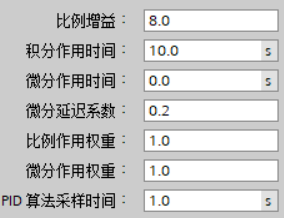
\includegraphics[width=.4\textwidth]{figure/串级-外环液位-模块-PID参数.PNG} 
    \caption{外环PID参数} % caption是图片的标题
    % \label{img} % 此处的label相当于一个图片的专属标志,目的是方便上下文的引用
\end{figure}
\begin{figure}[H]
    \centering % 居中 
    % 图片文件的相对路径
    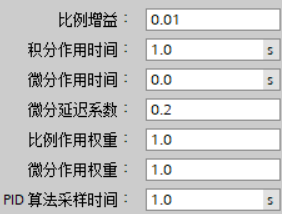
\includegraphics[width=.4\textwidth]{figure/串级-内环流量-模块-PID参数.PNG} 
    \caption{内环PID参数} % caption是图片的标题
    % \label{img} % 此处的label相当于一个图片的专属标志,目的是方便上下文的引用
\end{figure}

%%%
\subsubsection{控制效果展示}
主水箱液位-流量串级控制系统的控制效果展示如下:
\begin{figure}[H]
    \centering % 居中 
    % 图片文件的相对路径
    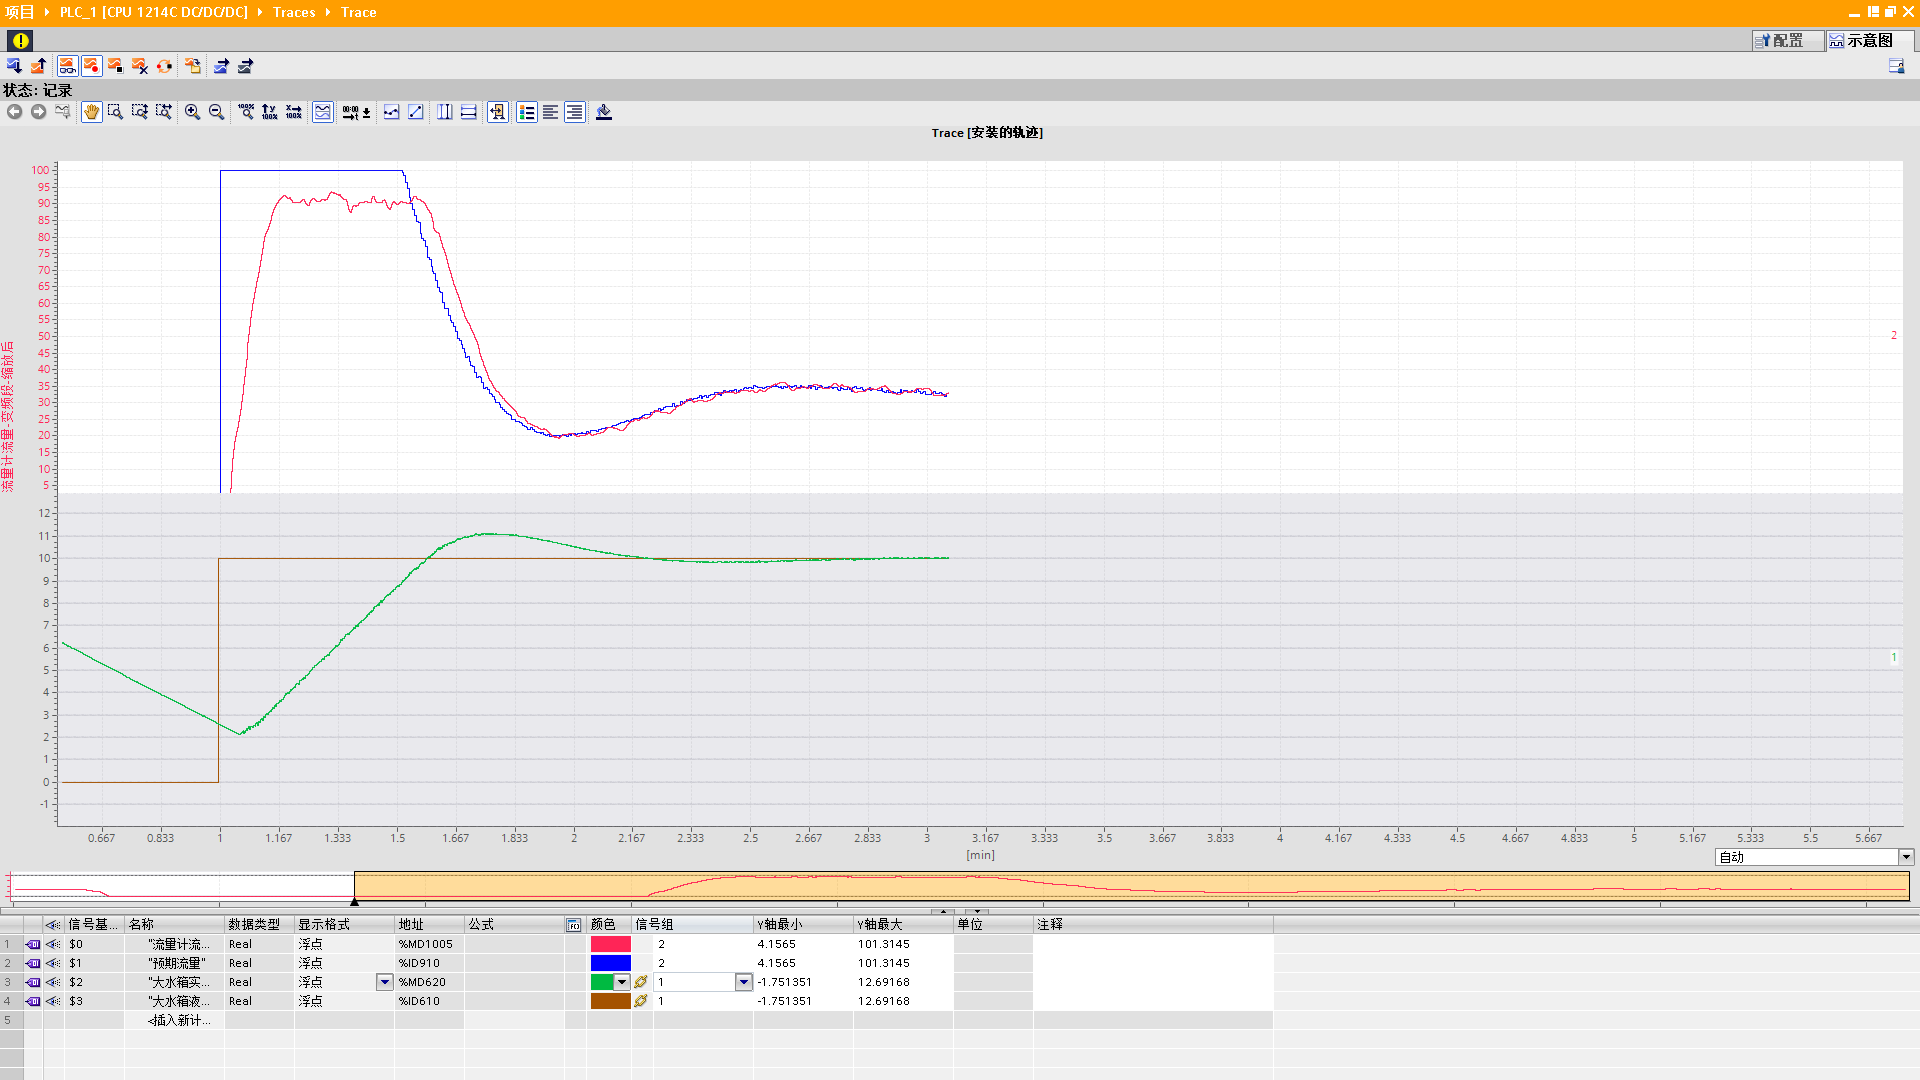
\includegraphics[width=1\textwidth]{figure/串级控制效果.png} 
    \caption{主水箱液位-流量串级控制系统效果} % caption是图片的标题
    % \label{img} % 此处的label相当于一个图片的专属标志,目的是方便上下文的引用
\end{figure}
可以看到,副回路所控制的管道流量基本上可以做到实时跟踪给定值,因此主水箱液位也能够以较好的方式稳定在给定值上,该串级系统整体上的控制效果是比较好的。

%%
\subsection{实验结论}
% 串级控制系统PID参数整定结果以及控制效果曲线参见上文所述内容。

在本次实验中,我们以双容水箱作为被控对象,设计了一个双容水箱液位串级控制系统。我们首先针对该串级控制系统的组成进行了分析,包括控制系统的被控对象、被控量、控制量、扰动量、所需的执行器和传感器等。然后基于以上分析构建了一个串级控制系统,并针对该控制系统的控制策略、控制器正反作用选取等问题展开了分析。此后我们基于工业中常用的的串级控制系统参数整定方法,对我们设计的系统进行了参数调试,并给出了最终的实验效果。

在这个过程中,我们学会了如何对复杂的控制对象和被控过程进行分析,掌握了串级控制系统的内外环结构构建和控制器设计方法,还学习了串级控制系统的参数整定方法。这些能力是自动化技术的基础部分,在我们的生活中被广泛地使用,相信在以后的学习和工作实践中有机会将它们应用于解决实际的问题。

\end{document}